\section{Data Analysis}
Our dataset consists of the daily open, high, low, close (OHLC) data for the time period 1999-01-01 through 2019-12-31 of the following major currency pairs
\begin{itemize}
    \item EURUSD - Euro € / U.S. Dollar \$
    \item GBPUSD - British Pound Sterling £ / U.S. Dollar \$
    \item USDCAD - U.S. Dollar \$ / Canadian Dollar \$
    \item USDJPY - U.S. Dollar \$ / Japanese Yen ¥
\end{itemize}
obtained from Dukascopy historical data feed~\cite{dukascopy}.
We will use the notation \( x_\text{open} \), \( x_\text{high} \), \( x_\text{low} \), and \( x_\text{close} \) to denote the open, high, low, and close values of a currency pair on a particular day.

Given that the values are on an absolute basis, we would like to convert them to relative terms in order to be able to compare data from different time periods on a more equal footing.
The natural way to do so is to compare the returns which are given by
\begin{align}
    r = \frac{x_\text{close} - x_\text{open}}{x_\text{open}}
\end{align}
However, this isn't necessarily the best way to approach this.
Instead we opt to use the log returns
\begin{align}
    \tilde{r}
        = \log(1+r)
        = \log\bigg( \frac{x_\text{close}}{x_\text{open}} \bigg)
\end{align}
due to several advantages~\cite{quantivity_2012}
\begin{itemize}
    \item Log-normality: if \( r \sim \mathcal{N}(\mu, \sigma^2) \) then \( \tilde{r} \sim \mathcal{N}(\tilde{\mu}, \tilde{\sigma}^2) \).
    \item Small \( r \) approximation: the expansion \( \log (1 + r) = r + \mathcal{O}(r^2) \approx r \) for \( r \ll 1 \).
    \item Time-additivity: instead of having to multiply one plus the returns to compound them, using log returns allows us to simply add them.
\end{itemize}

The first thing we need to do is to get an idea of how the log returns are distributed.
To get a visual overview we can analyze the histograms depicted in~\cref{fig:histograms_raw}.
From visual examination we see that the log returns are roughly normally distributed with the sample statistics given in~\cref{tbl:data_log_returns_raw_stats}.
\begin{figure}[!htb]
    \begin{center}
        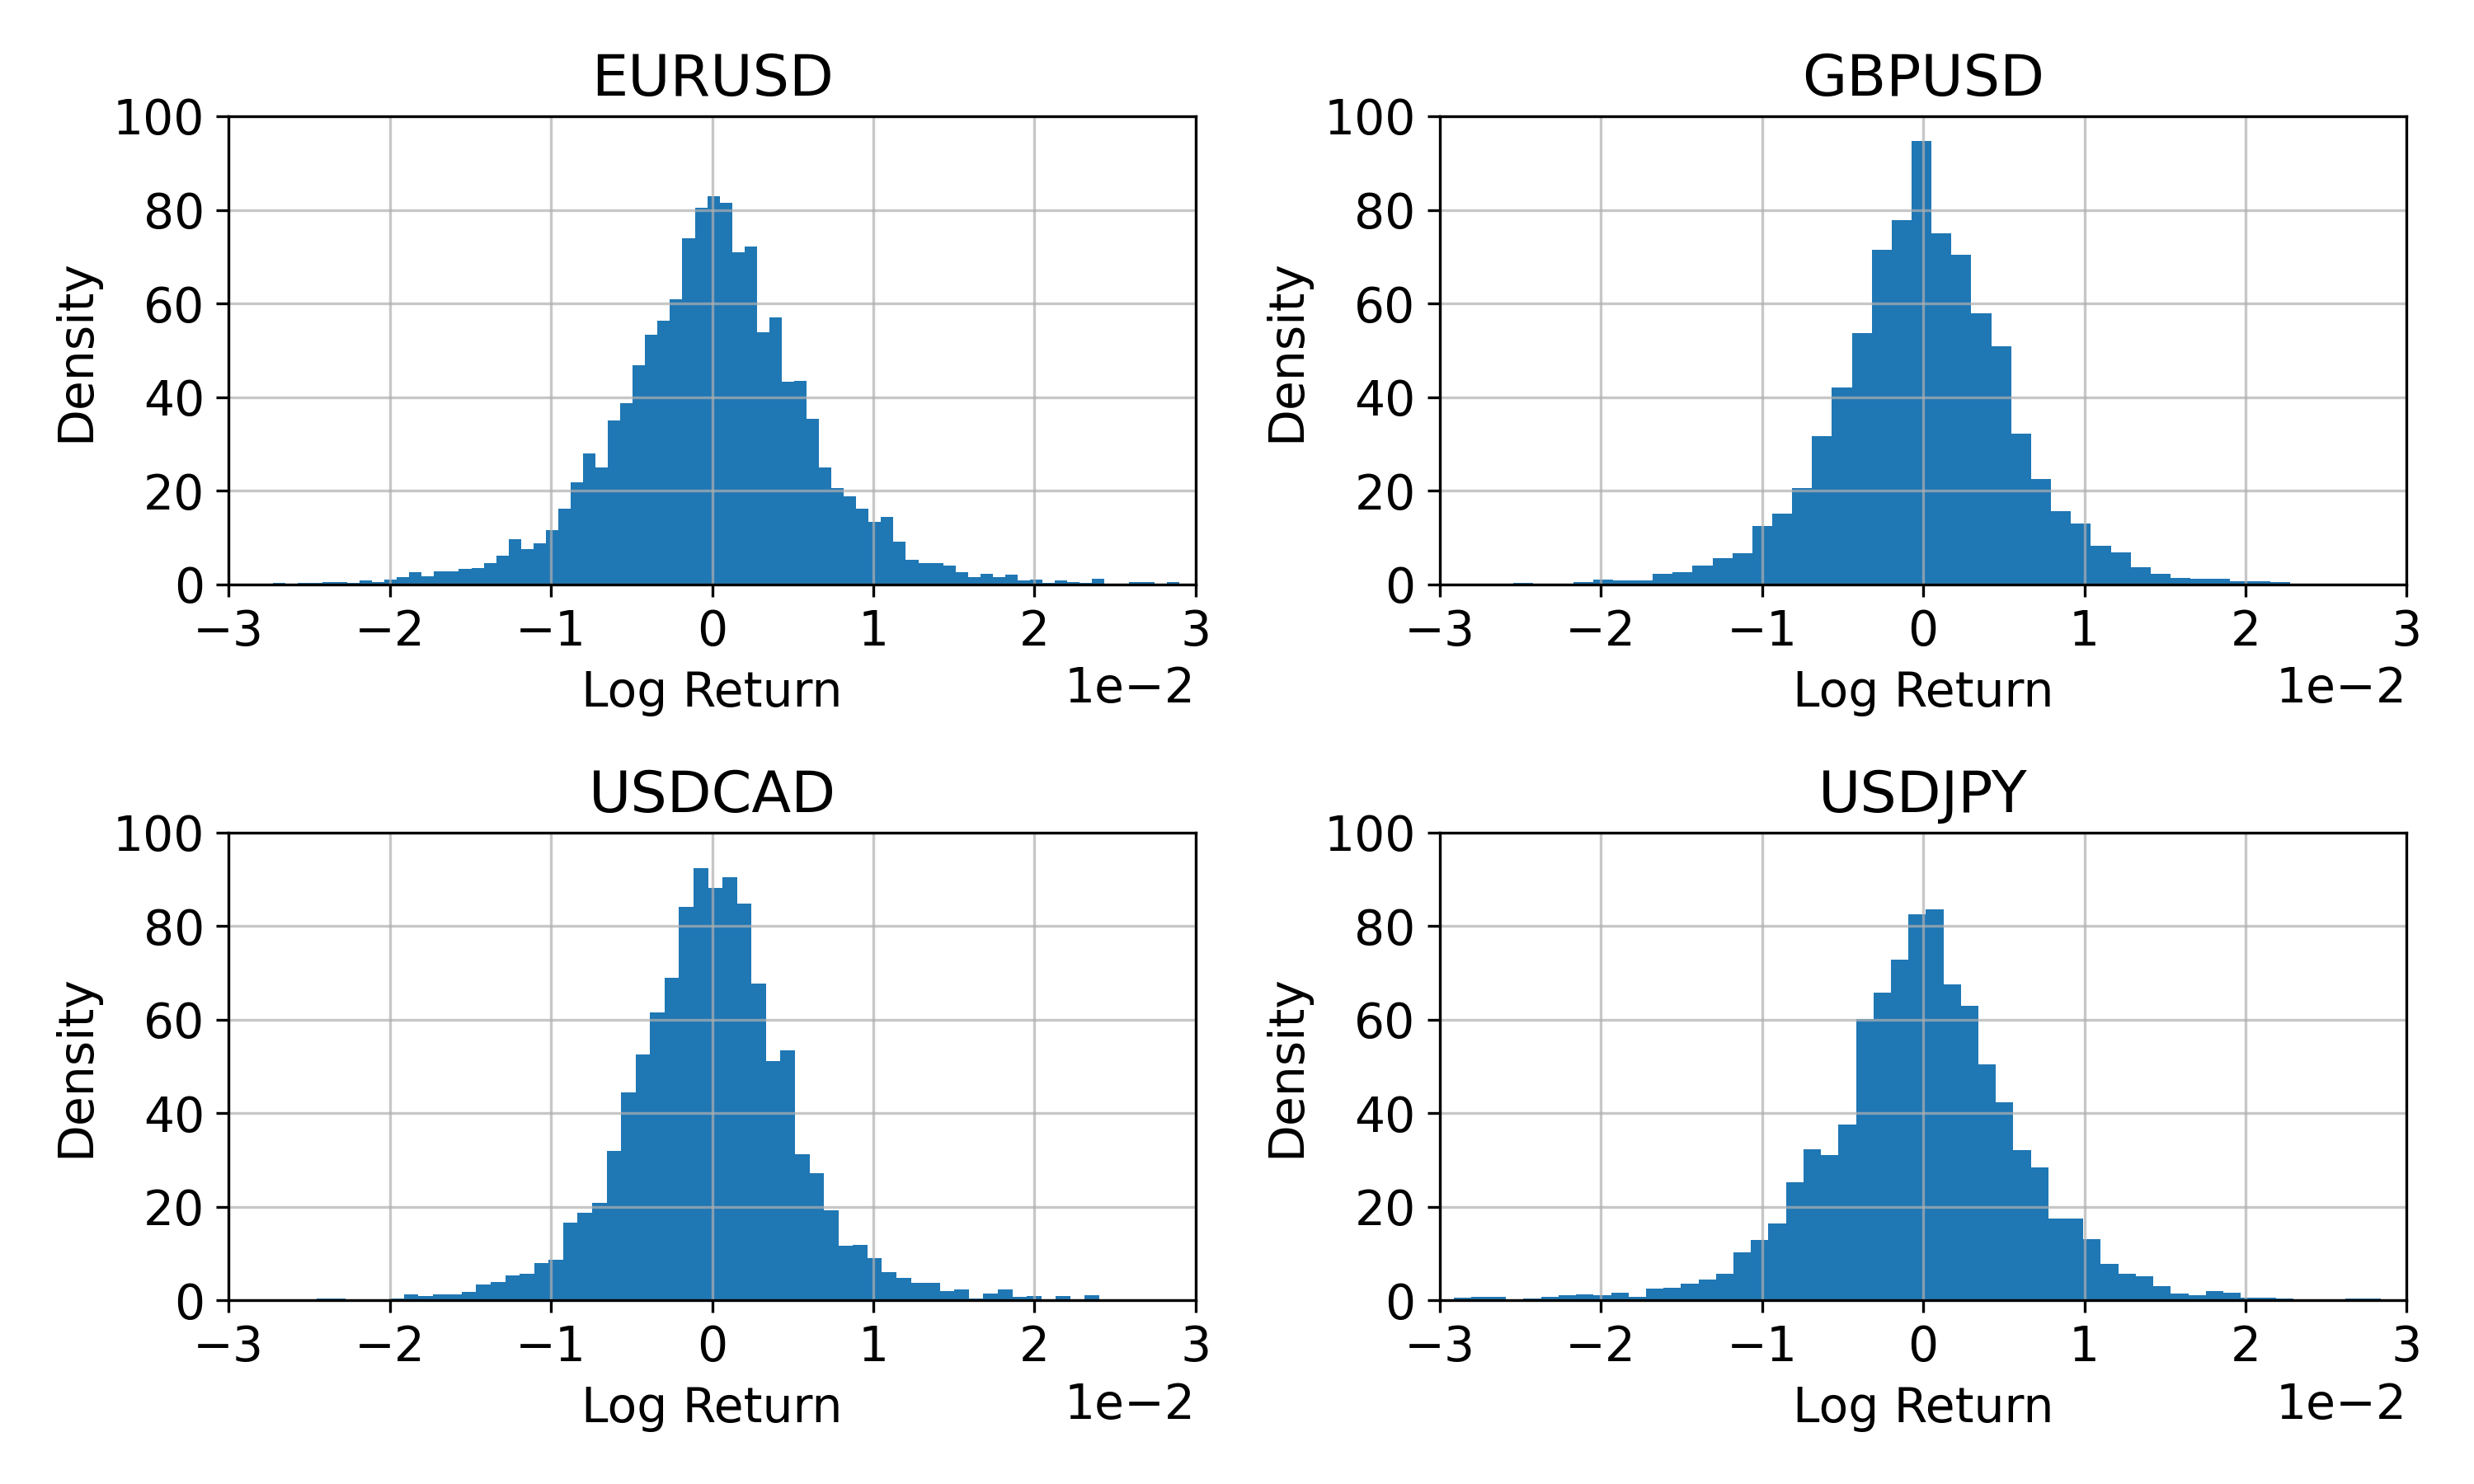
\includegraphics[width=1\linewidth]{data_analysis/histograms.png}
    \end{center}
    \caption{Histograms of the log returns of individual currency pairs exhibit Gaussian-like shapes around zero.}
    \label{fig:histograms_raw}
\end{figure}

\begin{table}[!htb]
    \centering
    \begin{adjustbox}{max width=\textwidth}
        \input{../tables/data/log_returns_raw_stats.tbl}
    \end{adjustbox}
    \caption{Sample statistics of the log returns.}
    \label{tbl:data_log_returns_raw_stats}
\end{table}

Another useful visualization to analyze the log returns is a violin/box plot, as shown in~\cref{fig:violin_raw}.
This allows us to identify outliers and see how they are distributed.
Immediately we see that there is one major outlier to the downside for the GBPUSD currency pair.
Further analysis indicates that this was an \( 11.1\sigma \) event occurring on 2016-06-24, which corresponds to the results of the Brexit referendum in the UK~\cite{brexit_gov_uk}.
The other outlier that really stands out is to the upside for the USDJPY currency pair on 2008-10-28.
This \( 8.3\sigma \) event occurred right in midst of the financial crisis when people were talking about the end of the Yen carry trade~\cite{jpy_carry_trade_nyt}.
\begin{figure}[!htb]
    \begin{center}
        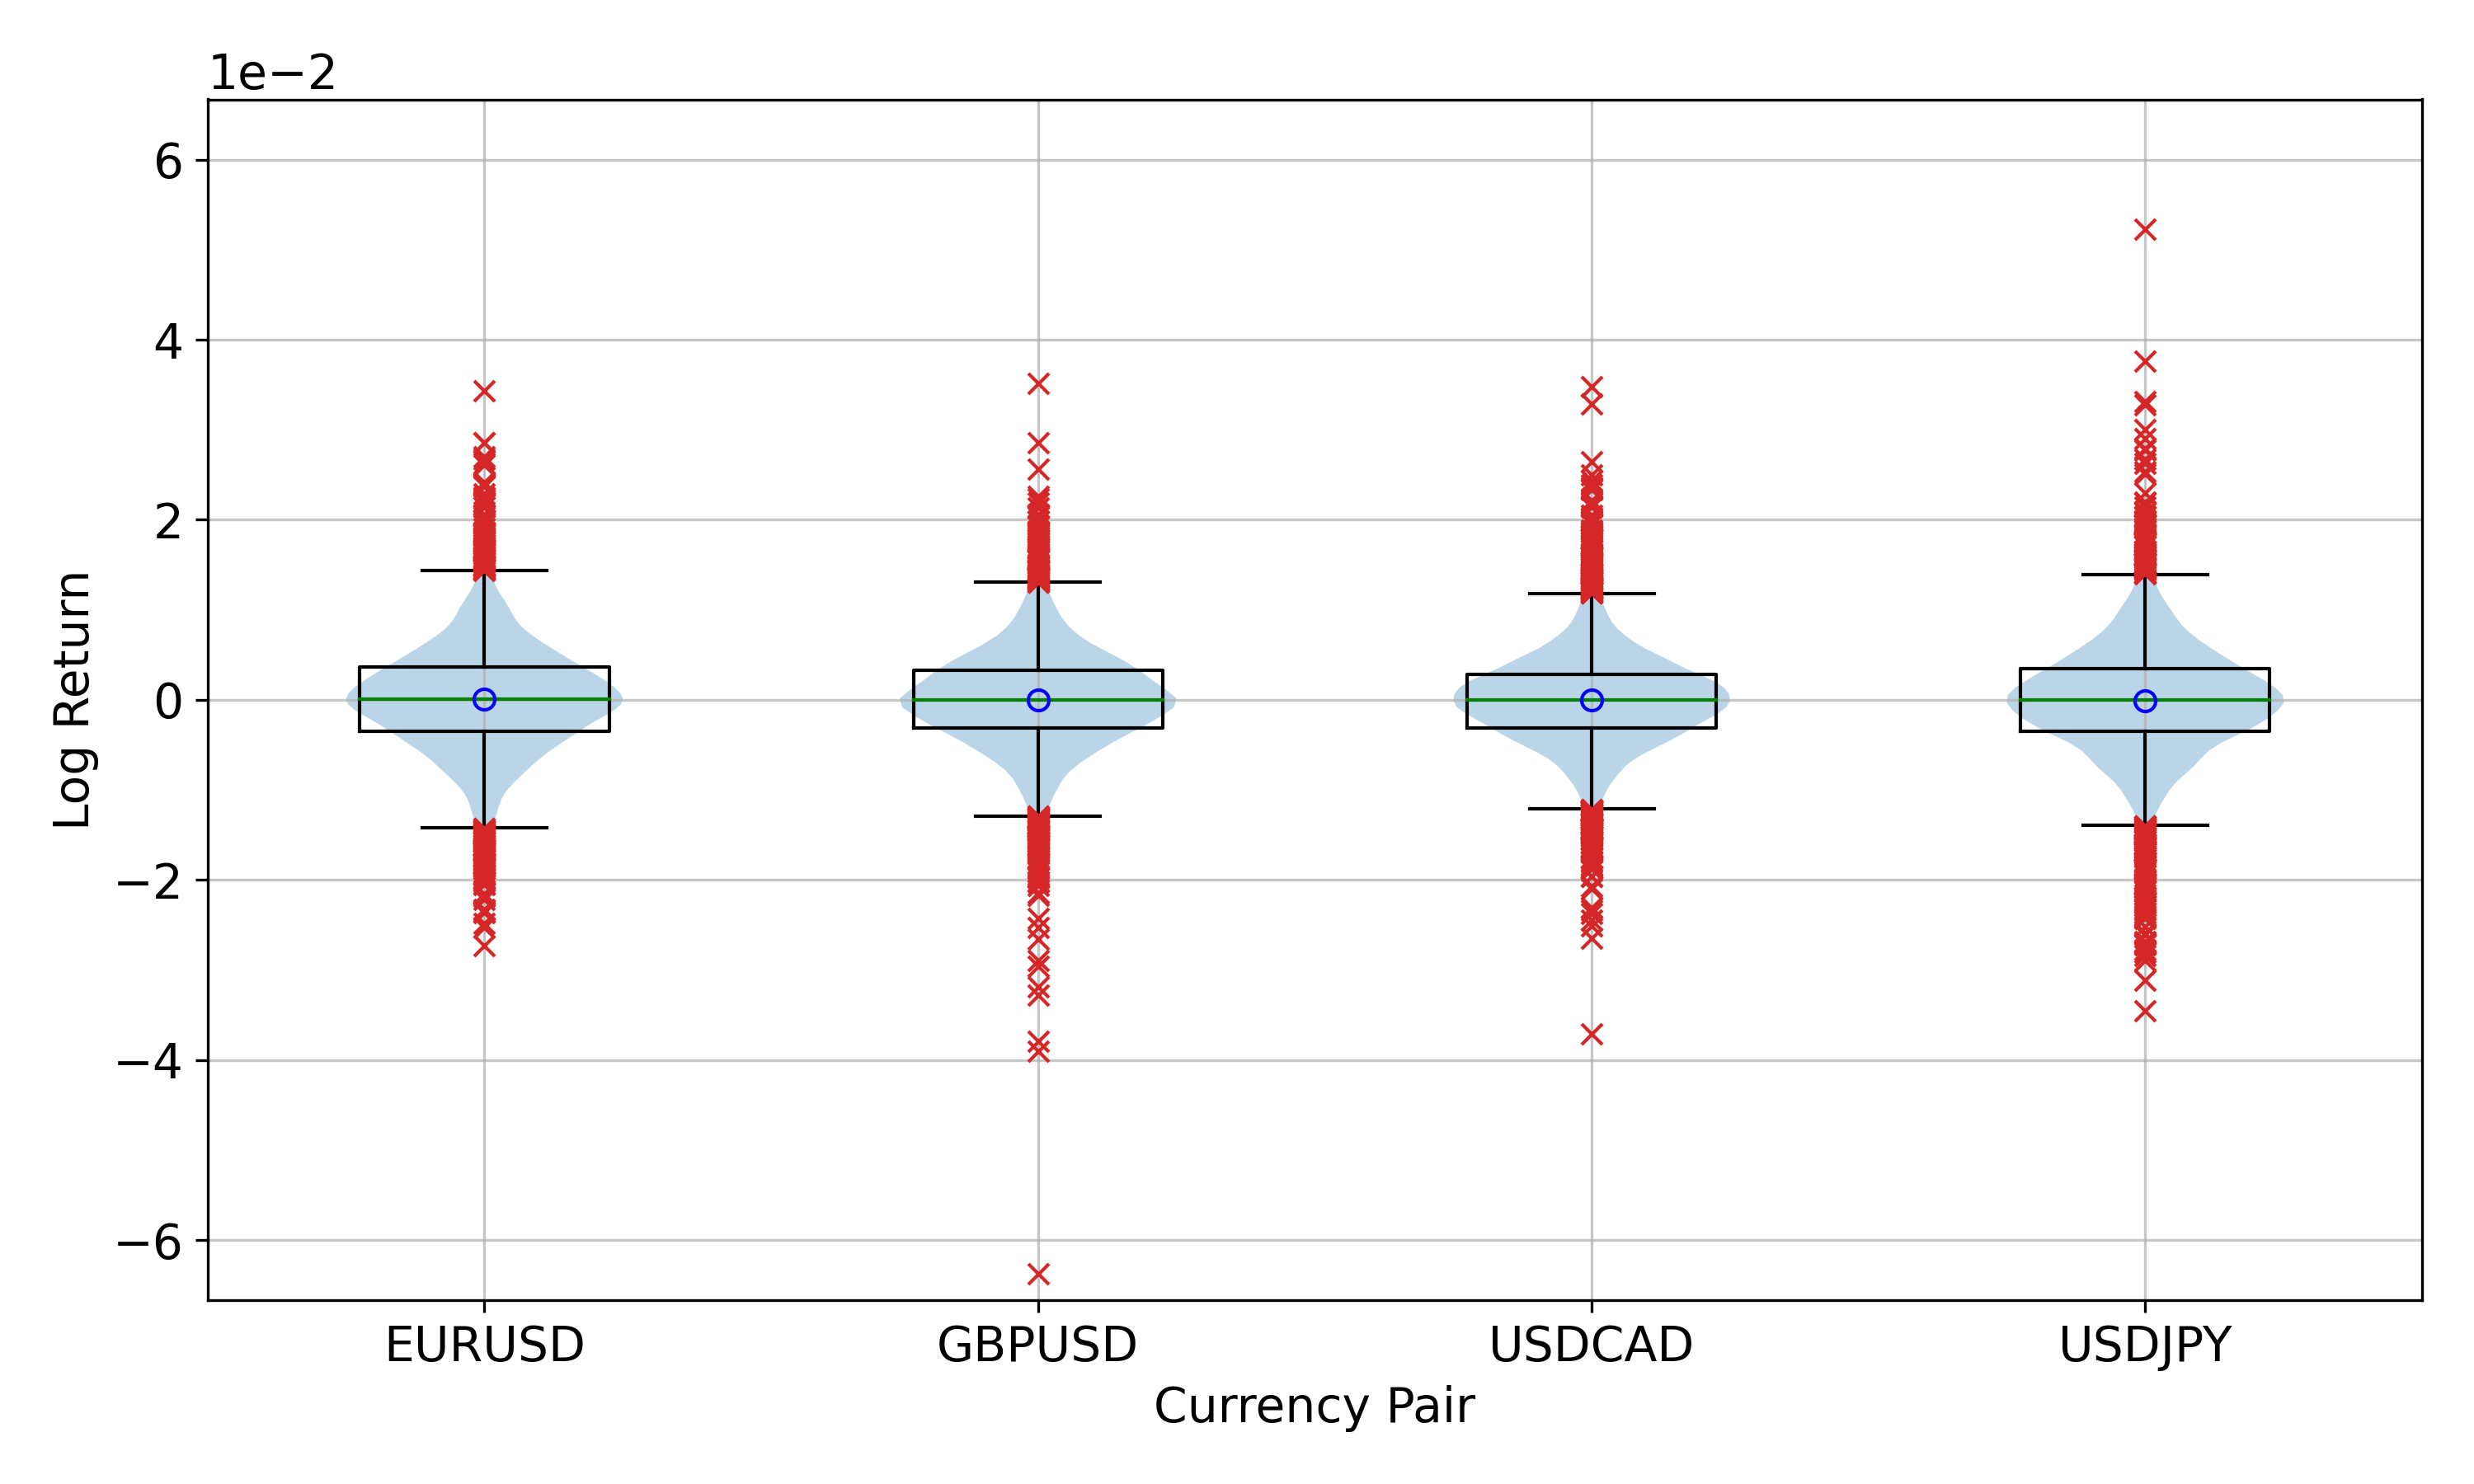
\includegraphics[width=1\linewidth]{data_analysis/violin.png}
    \end{center}
    \caption{Violin/box plot of the log returns for currency pairs show that there are two major outliers, one to the downside of GBPUSD and another to the upside of USDJPY.}
    \label{fig:violin_raw}
\end{figure}

Next we would like to analyze the correlations between the currency pairs to get an idea of the interdependencies between them.
This is visualized in~\cref{fig:scatters} where we see that there is a clear positive correlation between EURUSD/GBPUSD, and clear negative correlations between EURUSD/USDCAD and GBPUSD/USDCAD.
We verify this by examining the Pearson \( r \), Spearman \( \rho \), and Kendall \( \tau \) correlation coefficients laid out in~\cref{tbl:data_correlation_coefficients}.
The correlation coefficients are positive when the pairs are of the form \( X \)USD/\( Y \)USD, and negative when the pairs are of the form \( X \)USD/USD\( Y \), for \( X,Y \in \) \{EUR, GBP, CAD, JPY\}.
\begin{figure}[!htb]
    \begin{center}
        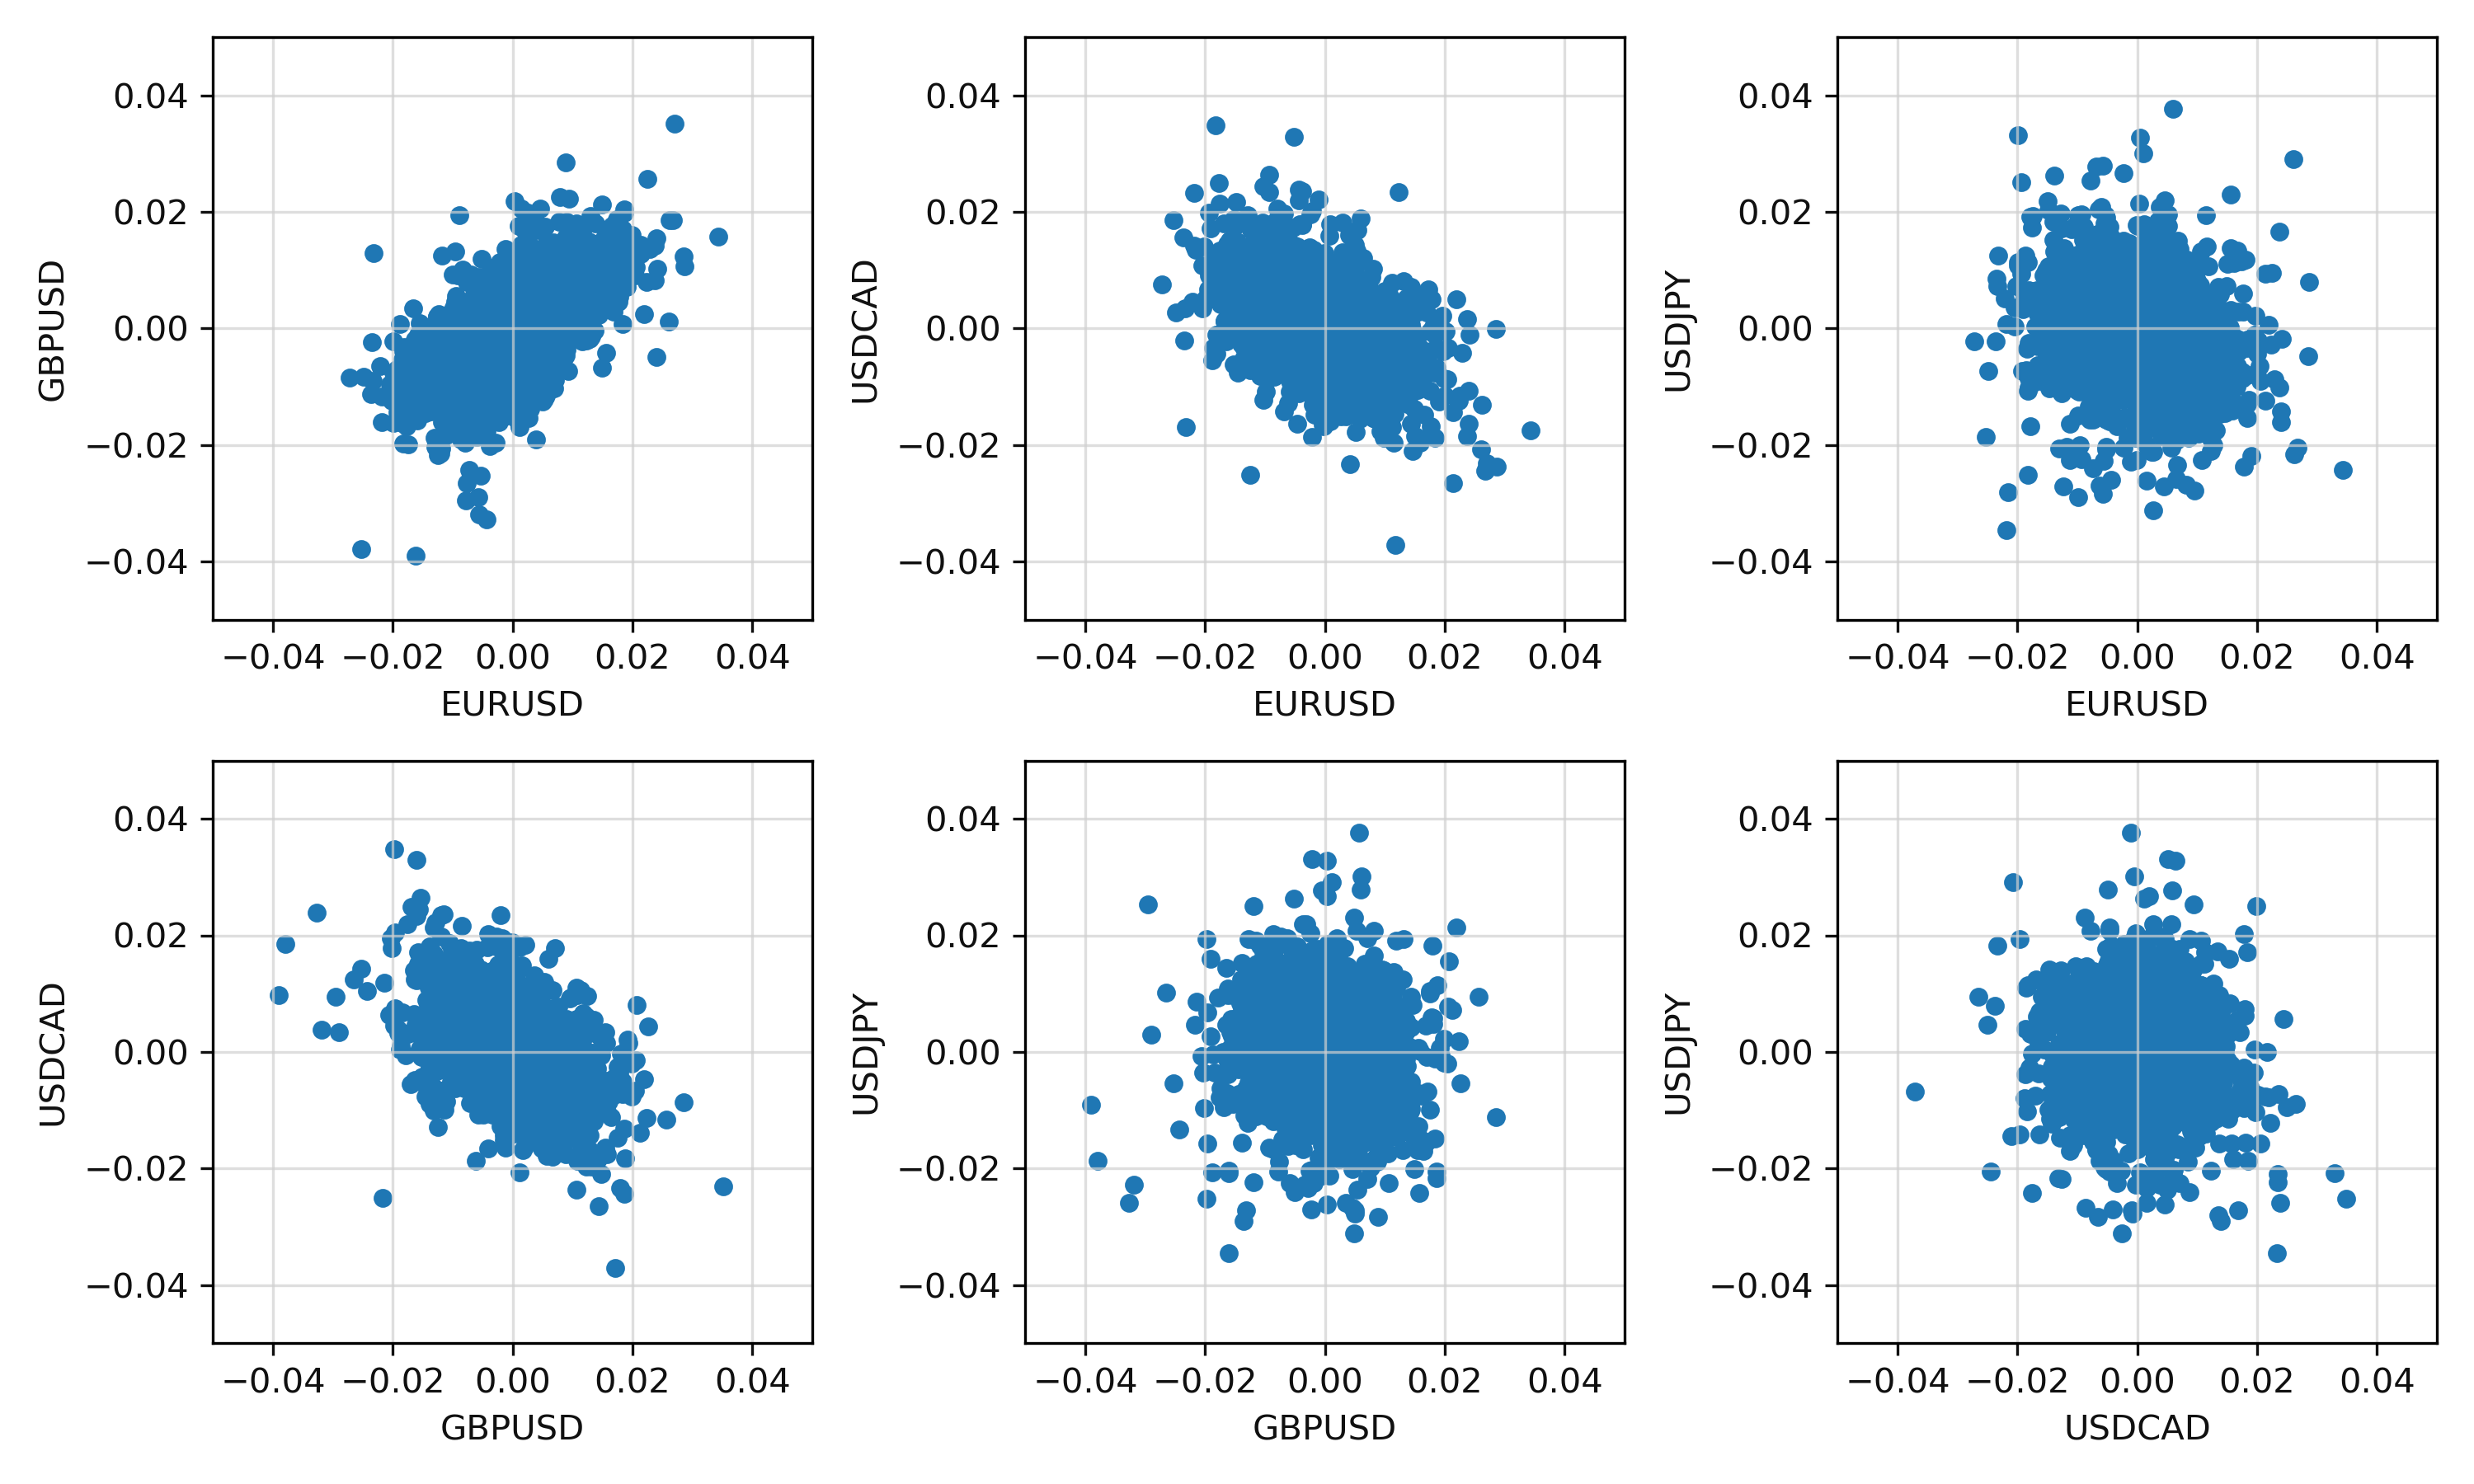
\includegraphics[width=1\linewidth]{data_analysis/scatters.png}
    \end{center}
    \caption{The scatter matrix of the currency pairs shows a clear positive correlation between EURUSD/GBPUSD, and clear negative correlations between EURUSD/USDCAD and GBPUSD/USDCAD.}
    \label{fig:scatters}
\end{figure}

\begin{table}[!htb]
    \centering
    \begin{adjustbox}{max width=\textwidth}
        \input{../tables/data/correlation_coefficients.tbl}
    \end{adjustbox}
    \caption{Correlation coefficients of the currency pairs.}
    \label{tbl:data_correlation_coefficients}
\end{table}


\section{Data Preprocessing}
In order to feed the data to the models in the following sections, we first need to convert the data to a form in which it is represented by binary vectors.
Let \( \mat{X} \in \R^{4 \times N} \) represent the training dataset of log returns, where training examples are vectors in the column space, thus element \( x_{ij} \) represents the \( i \)th currency pair log return for the \( j \)th training example.

When binarizing the data, we first rescale the entries of \( \mat{X} \) to integer values in \( \{0, 1, \dots, 2^{n_\text{bits}} - 1\} \), represented by the matrix \( \mat{X}' \in \N^{4 \times N} \) with entries
\begin{align}
    x_{ij}' = \bigg\lfloor \frac{x_{ij} - \min_k x_{ik}}{\max_k x_{ik} - \min_k x_{ik}} \cdot (2^{n_\text{bits}} - 1) \bigg\rceil
\end{align}
where \( \lfloor \ \cdot \ \rceil \) denotes rounding to the nearest integer.

After we have the integer values we create a new matrix \( \mat{V} \in \binset^{4\cdot n_\text{bits} \times N} \) where the columns of \( \mat{V} \) are the \( n_\text{bits} \)-length binary representation vectors of the entries of the columns of \( \mat{X}' \) concatenated together.
For example, if \( \vec{x} = (x_1,x_2,x_3,x_4) \) is a column of \( \mat{X} \), and the function \( \text{bin}(x) \) takes in an integer \( x \) and returns a binary column vector, then the corresponding column in \( \mat{V} \) would be
\begin{align}
    \vec{v} = \begin{bmatrix}
        \text{bin}(x_1) \\
        \text{bin}(x_2) \\
        \text{bin}(x_3) \\
        \text{bin}(x_4) \\
    \end{bmatrix}
\end{align}

For the dataset at hand we use \( n_\text{bits} = 16 \), which gives us a training set \( \mat{V} \in \binset^{64 \times N} \), thus our training examples are binary vectors of length 64.
The discretization errors associated with this conversion and dataset are on the order \( 10^{-7} \), which is within the desired tolerance for this purpose.

\subsection{Data Transformation}
Due to how the data is converted linearly to a binary form, data with outliers can have a "gap" between large outliers and the next closest value, which can lead to difficulties in training.
To mitigate this, we create a transformation to reduce this gap by scaling outliers beyond a certain threshold \( \tau \), as detailed in~\cref{alg:transformation}.
In practice we take \( \tau = 1 \) and \( \alpha = 0.5 \), thus the standardized data points above one standard deviation are mapped to their square root, this case is illustrated in~\cref{fig:data_transformation}.
This transformation is reversible if we save \( \overline{x} \), \( \sigma_x \), and \( \delta \).

Of course this transformation doesn't necessarily have an inherent meaning, and the transformed data isn't necessarily representative of anything, but this was found to improve some of the model results as we will see in the next chapter.

\begin{algorithm}
    \caption{Outlier Power Transformation}
\begin{algorithmic}[1]
    \Procedure{Transform}{$\vec{x}, \alpha, \tau$}
            \Comment $\alpha$ is the power, $\tau$ is the threshold
        \State $\overline{x} \gets \text{mean}(\vec{x})$
        \State $\sigma_{x} \gets \text{std}(\vec{x})$
        \State $\delta \gets \tau - \tau^\alpha$
            \Comment ensures the transformation is reversible
        \For {$i$ in 1 to length($\vec{x}$)}
            \State $x_i \gets (x_i - \overline{x}) / \sigma_x$
                \Comment standardize
            \If {$x_i \ge \tau$}
                \State $x_i \gets (\abs{x_i}^\alpha + \delta) \cdot \text{sign}(x_i)$
                    \Comment scale standardized values beyond $\tau$
            \EndIf
            \State $x_i \gets x_i \cdot \sigma_x + \overline{x}$
                \Comment undo standardization
        \EndFor
    \EndProcedure
\end{algorithmic}
\label{alg:transformation}
\end{algorithm}

\begin{figure}[!htb]
    \begin{center}
        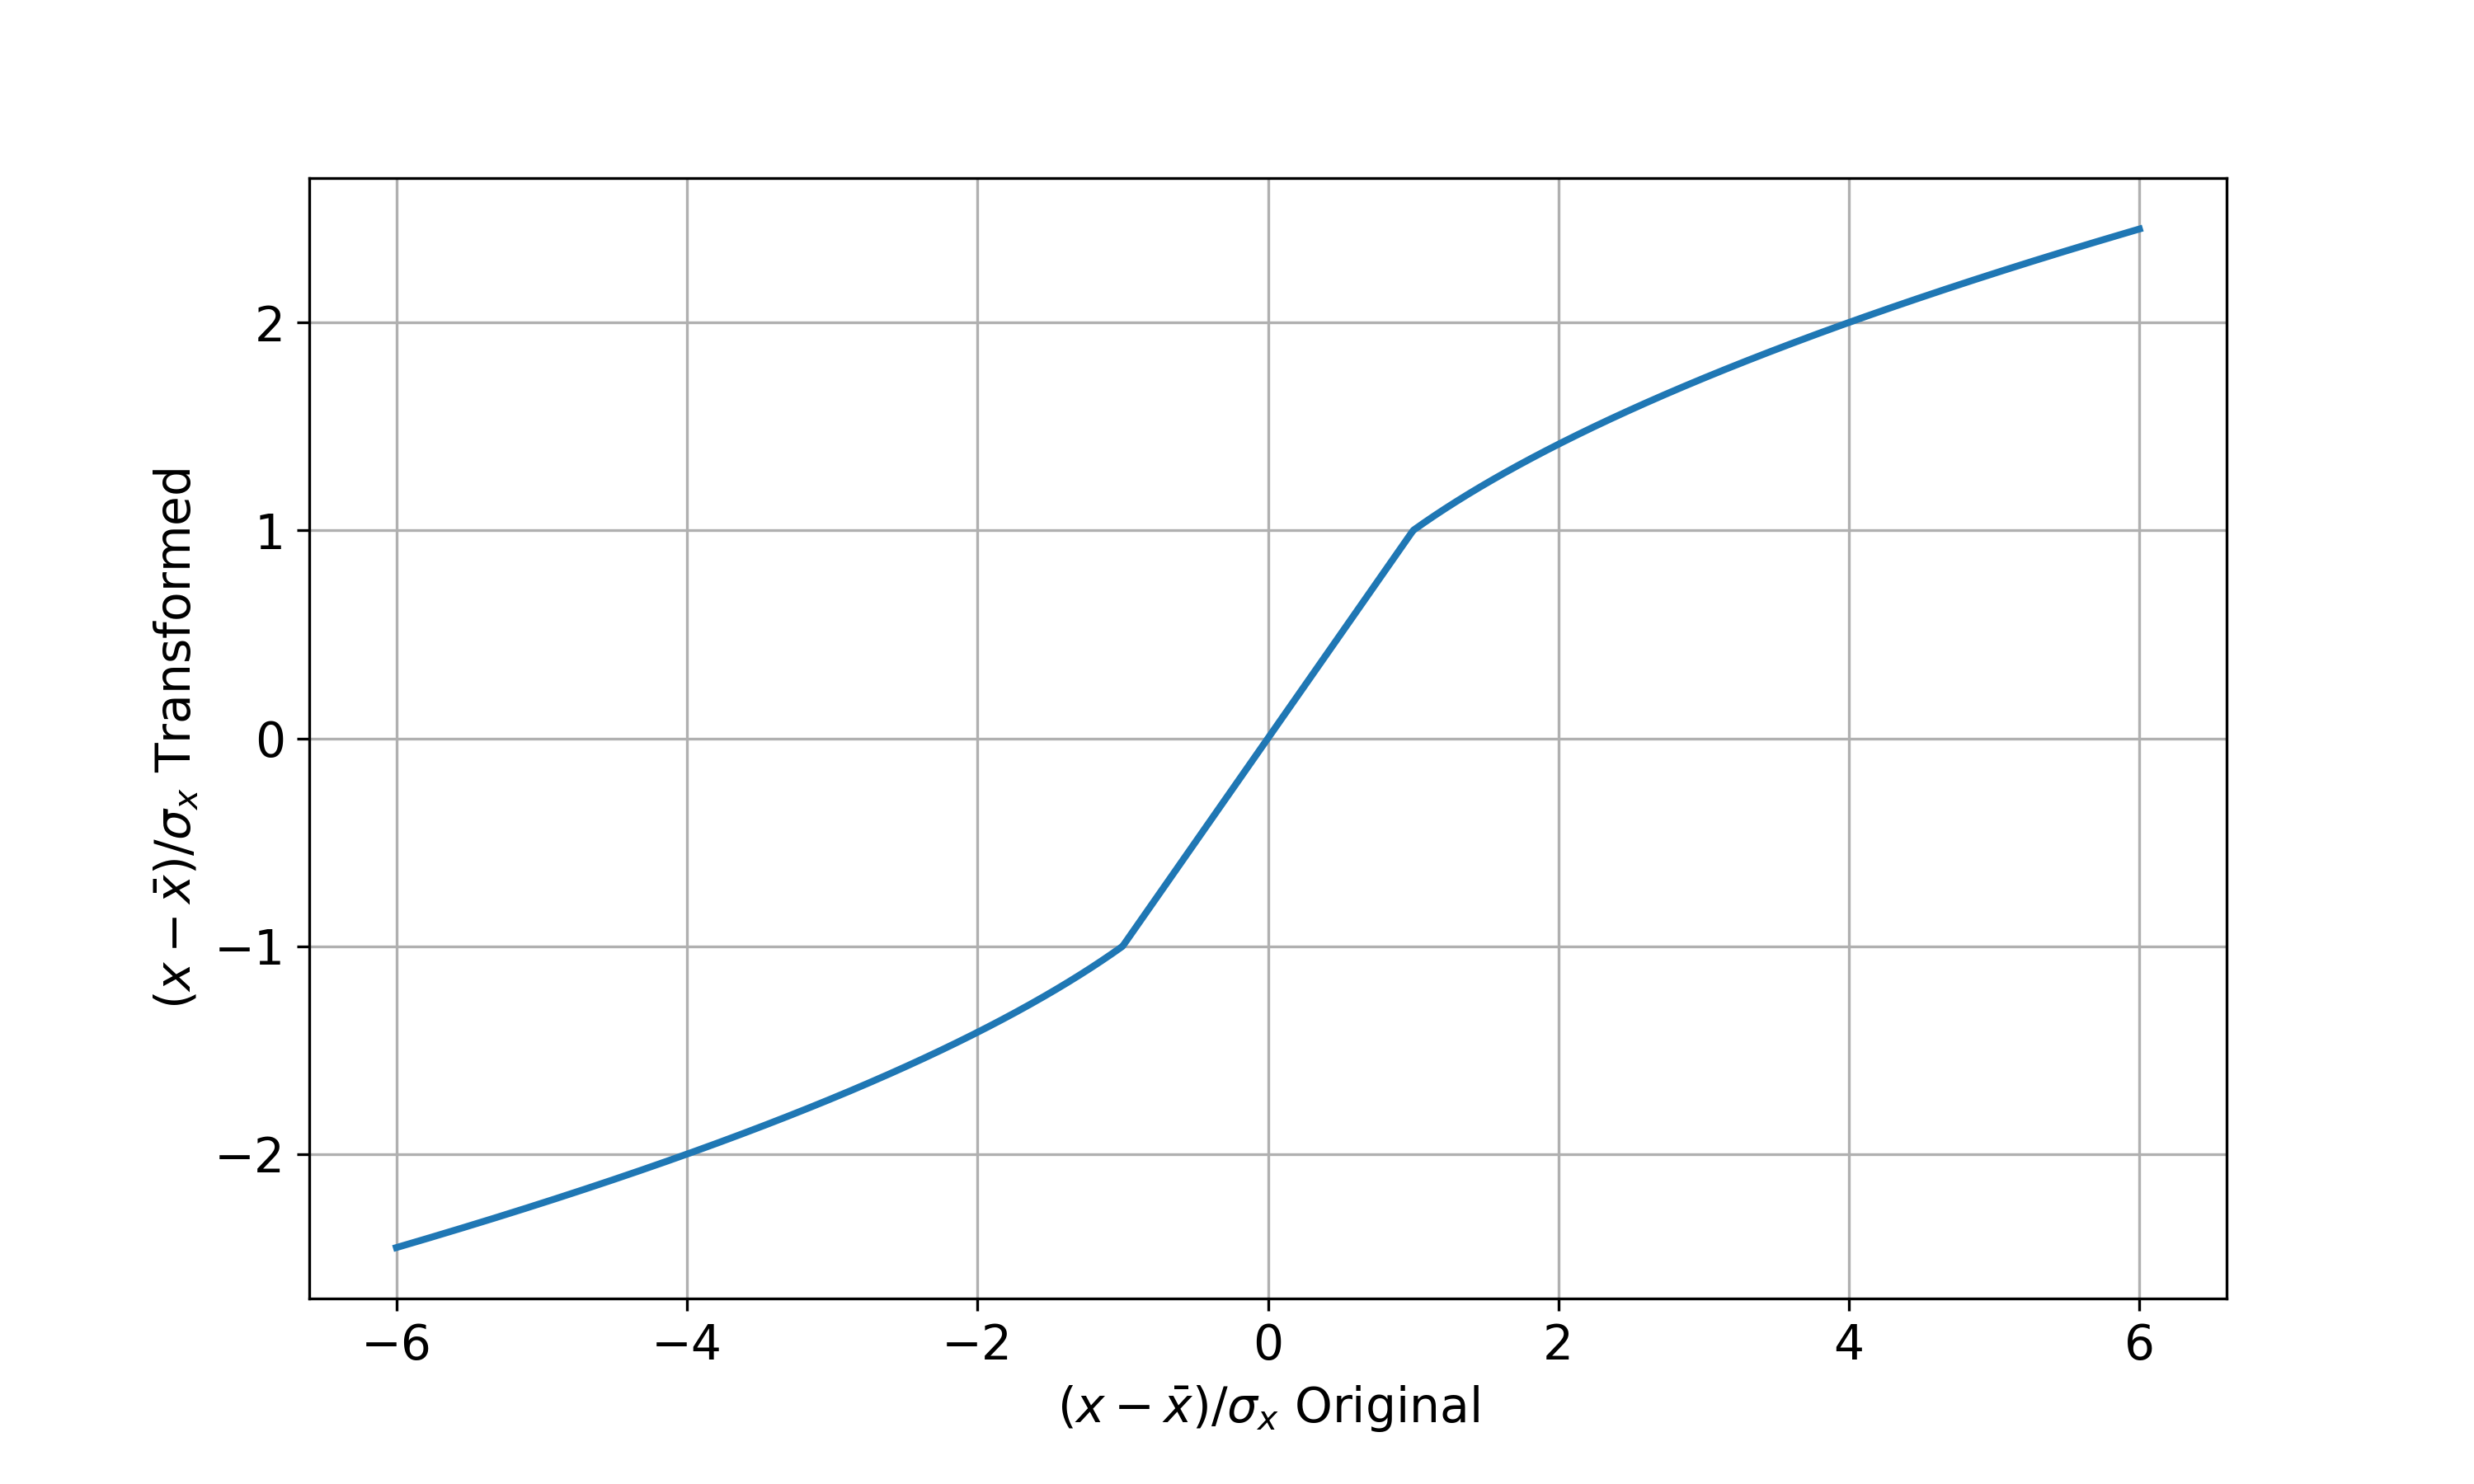
\includegraphics[width=1\linewidth]{data_analysis/data_transformation.png}
    \end{center}
    \caption{Transformation applied to the data before training using \( \tau = 1 \) and \( \alpha = 0.5 \), for the purpose of reducing large "gaps" in the binarized data by scaling outliers above one standard deviation by taking the square root of their standardized value.}
    \label{fig:data_transformation}
\end{figure}

In~\cref{fig:data_transformation} we see the outlier power transformation applied to the log returns training data.
This brings in the outliers and creates "shoulders" on the Gaussian shaped histograms.
As expected, the violin and box plot in~\cref{fig:violin_transformed} shows the transformed data has significantly less outliers, and \cref{tbl:data_log_returns_transformed_stats} shows that the standard deviations have been decreased relative to the originals given in~\cref{tbl:data_log_returns_raw_stats}.

\begin{figure}[!htb]
    \begin{center}
        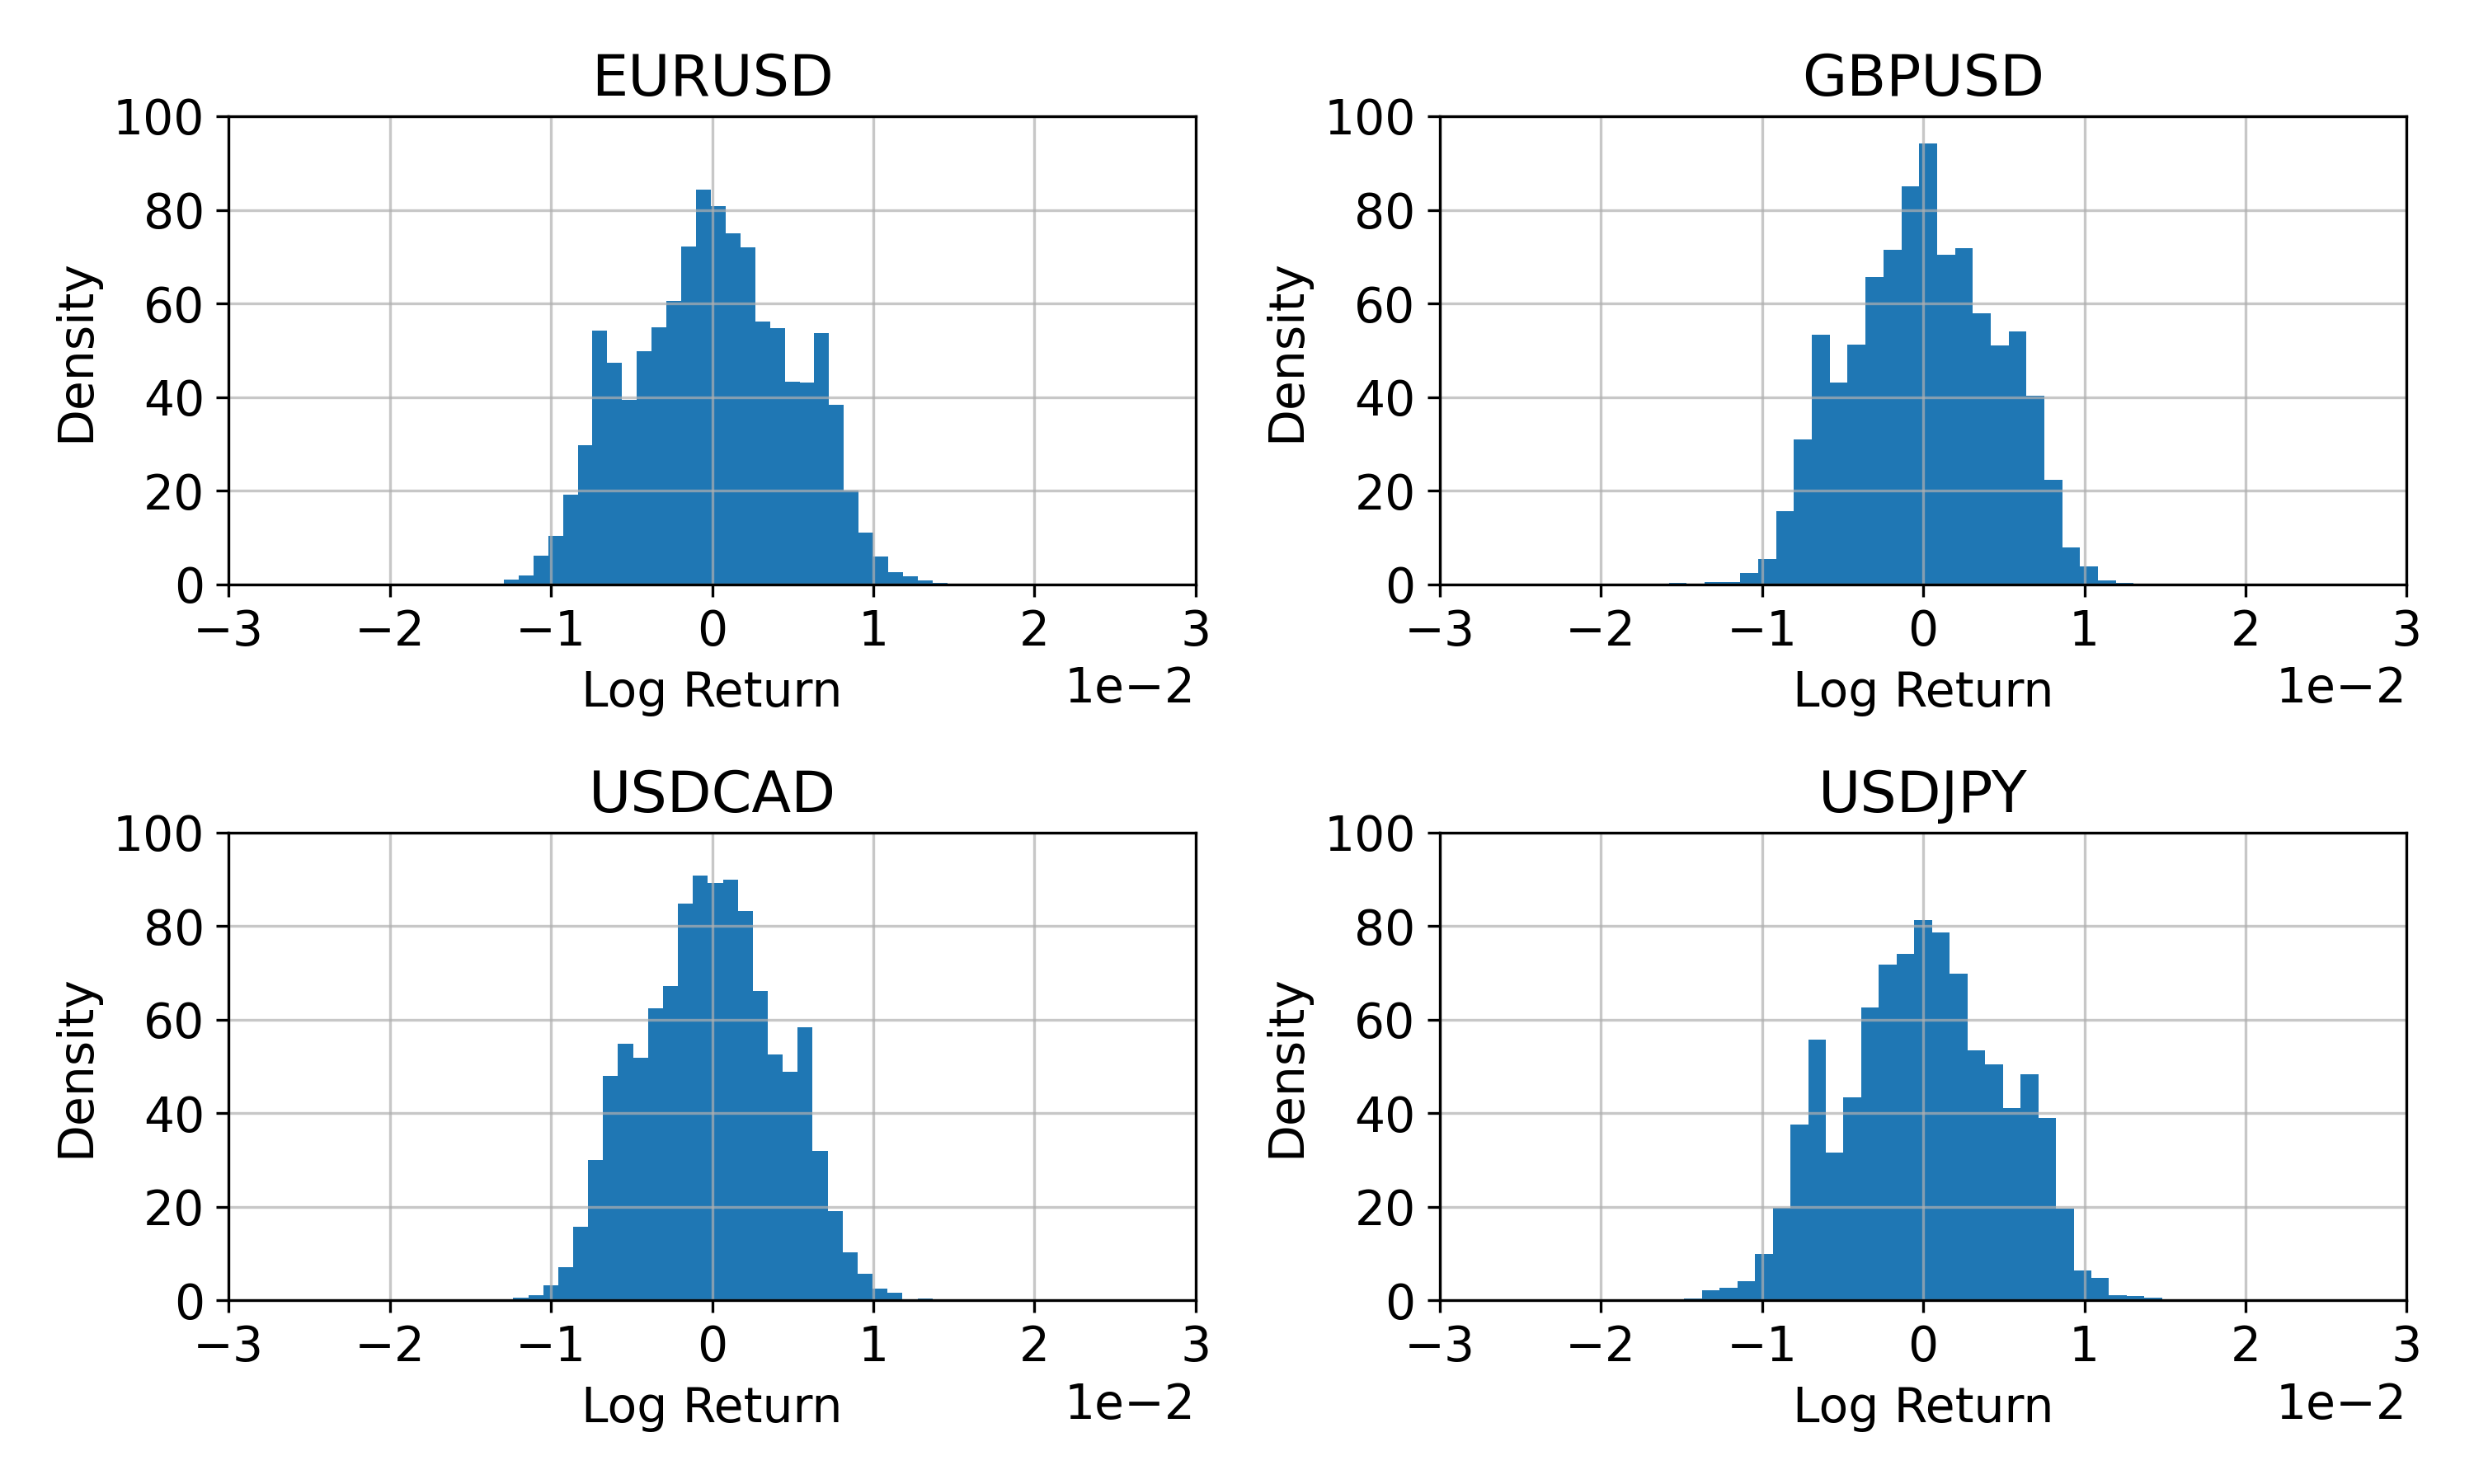
\includegraphics[width=1\linewidth]{data_analysis/histograms_transformed.png}
    \end{center}
    \caption{Histograms of the transformed log returns of currency pairs have shoulders around the threshold \( \tau \) which do not appear in the original.}
    \label{fig:histograms_transformed}
\end{figure}
\begin{figure}[!htb]
    \begin{center}
        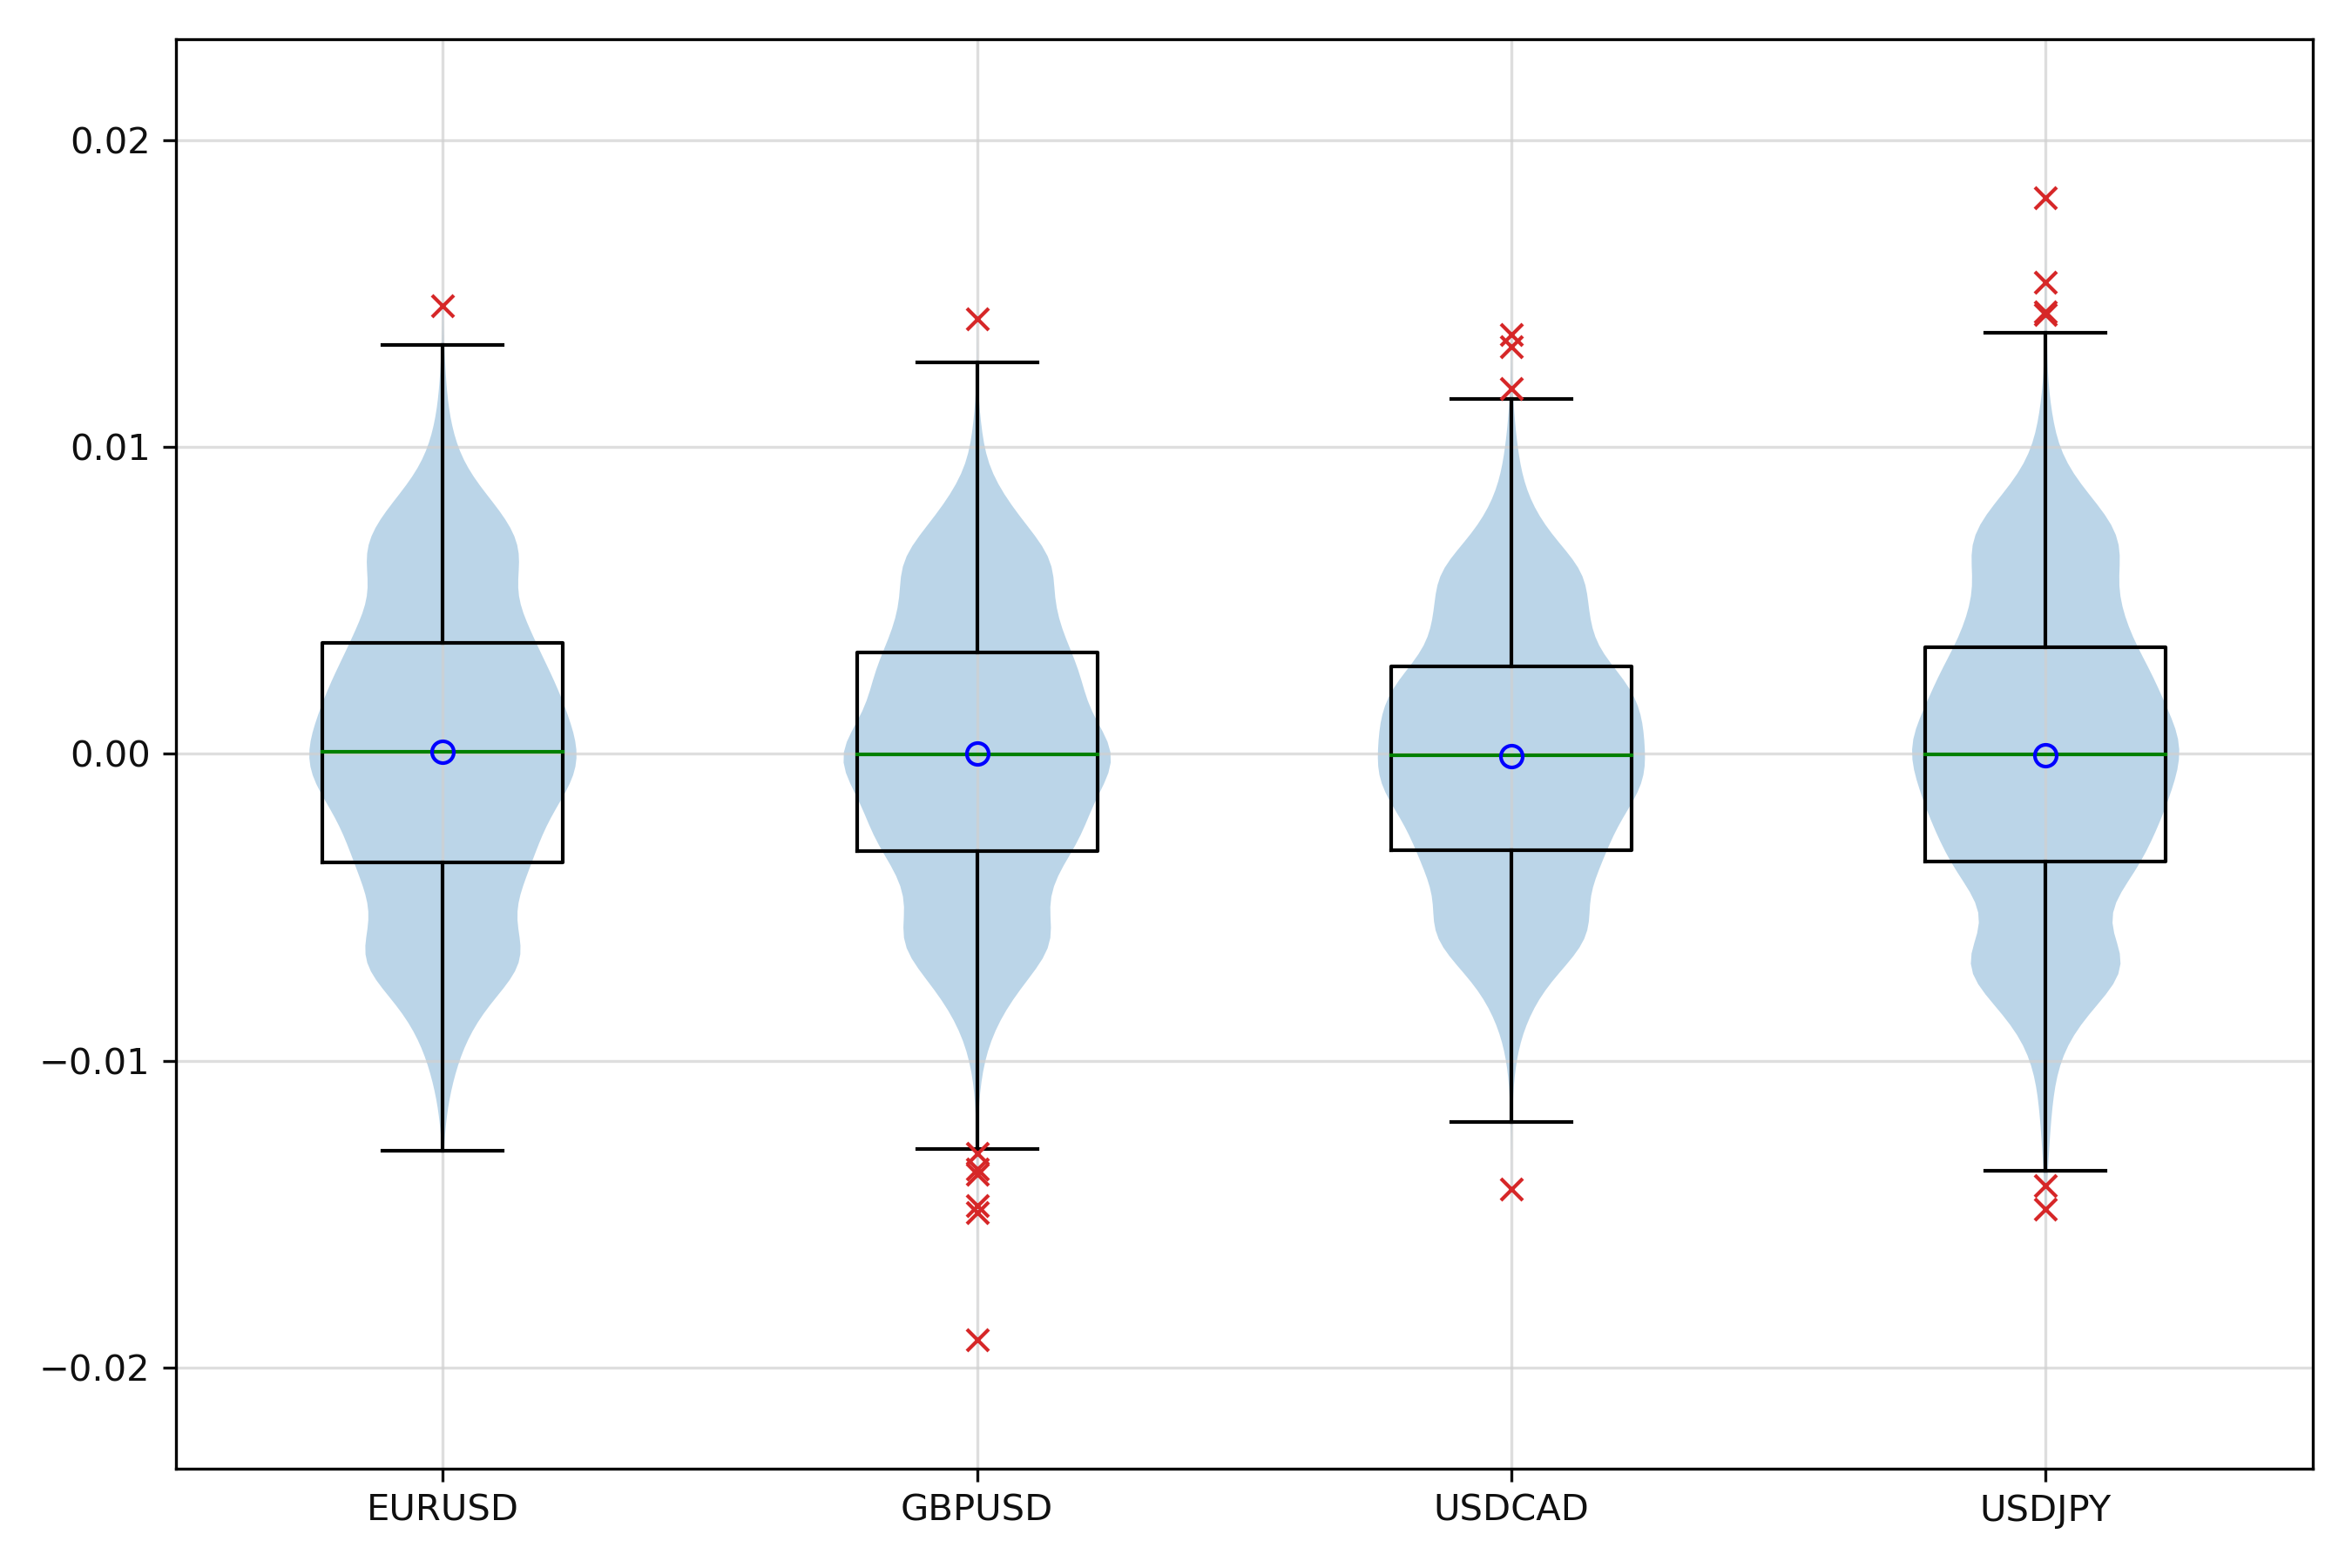
\includegraphics[width=1\linewidth]{data_analysis/violin_transformed.png}
    \end{center}
    \caption{Violin/box plot of the transformed log returns for currency pairs shows how the outliers have been scaled closer to the mean.}
    \label{fig:violin_transformed}
\end{figure}
\begin{table}[!htb]
    \centering
    \begin{adjustbox}{max width=\textwidth}
        \input{../tables/data/log_returns_transformed_stats.tbl}
    \end{adjustbox}
    \caption{Sample statistics of the transformed log returns.}
    \label{tbl:data_log_returns_transformed_stats}
\end{table}

\subsection{Additional Information}
We can increase the information content of the training data by adding additional variables.
One such bit of information is the rolling volatility relative to the historical median.
In finance we compute the annualized volatility of a time series vector \( \vec{x} \) as
\begin{align}
    \text{vol}(\vec{x}) = \sqrt{252} \cdot \text{std}(\vec{x})
\end{align}
where the factor of \( \sqrt{252} \) comes from the square root of the number of trading days in a year, i.e., it's the annualization factor.
In \cref{fig:rolling_volatility} we show the 3-month rolling volatility versus its historical median which indicates whether it's in the low or high volatility regime.

We can encode this data as additional binary indicators that are one when above the historical median, and zero when below.
This can then be concatenated onto the training data and fed to the model to make it more flexible by allowing for the results to be conditioned on a specific volatility regime.
Adding one such indicator for each currency increases the number of rows in our training dataset by four, thus the concatenated dataset lies in the space \( \binset^{68 \times N} \).

\begin{figure}[!htb]
    \begin{center}
        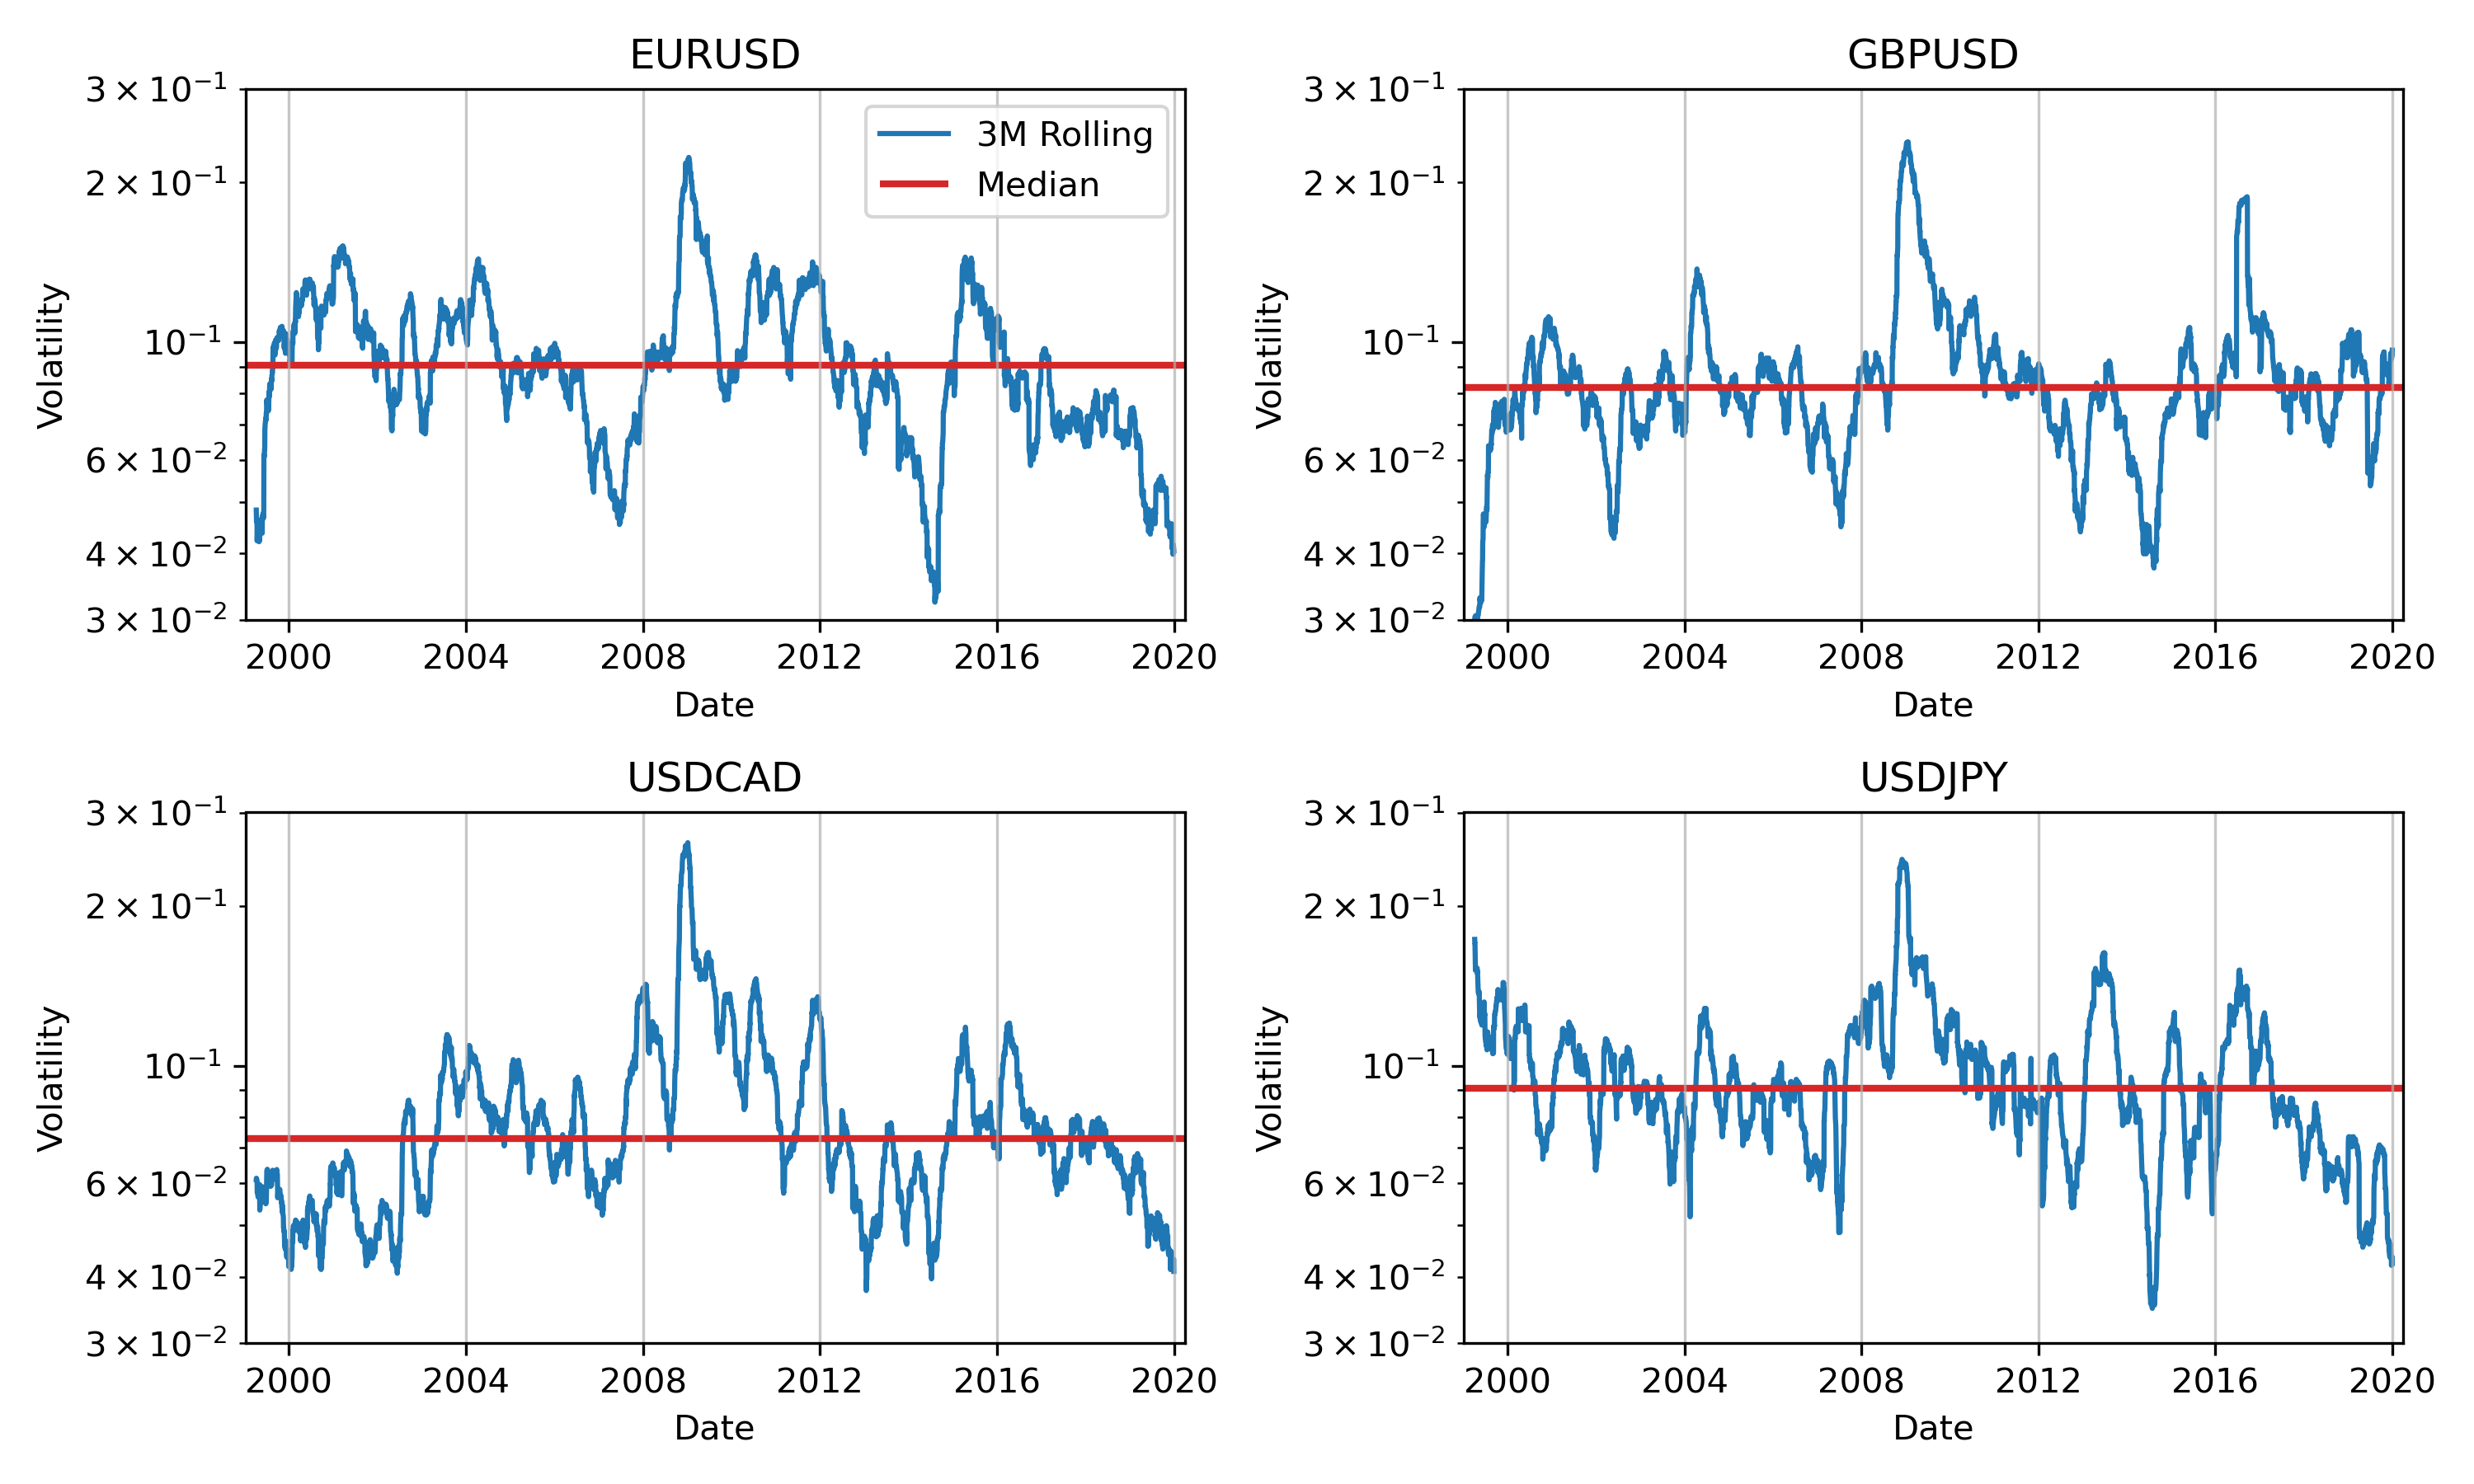
\includegraphics[width=1\linewidth]{data_analysis/rolling_volatility.png}
    \end{center}
    \caption{3-month rolling volatility of the log returns for currency pairs compared to the historical median.}
    \label{fig:rolling_volatility}
\end{figure}
